\chapter{NUMA Topology Views}
Kapitola se bude zabývat posledním z hlavních vylepšení této práce, tj. přidáním informací o NUMA topologii CPU na systému do KernelSharku. Tato modifikace pak bude hlavně sloužit k vylepšení analýzy trasovacích dat, jelikož budeme jednodušeji schopni určit namáhanou část topologie. Kapitola postupně představí cíle, analýzu řešení, návrh, uživatelskou dokumentaci, návrhy pro rozšíření, kritiku řešení a konečné zhodnocení splnění cílů této modifikace.

%%%%%%%%%%%%%%%%%%%%%%%%%%%%%%%%%%%%%%%%%%%%%%%%%%%%%%%%%%%%%%%%%%%%%%%
\section{Cíle}

\begin{itemize}
    \item Modifikace bude umět zpracovat topologická data z XML souboru vytvořeného programem Hwloc. Z tohoto souboru bude hlavně chtít vyčíst NUMA topologii procesorů.
    \item Zpracovaná topologická data budou zobrazena někde v hlavním okně. Místo zobrazení by mělo dovolovat přirozenou návaznost na CPU grafy. Ty mohou být přeuspořádány tak, aby respektovaly řazení v topologii.
    \item Pokud nemáme topologická data k dispozici pro nějaký stream, nebudeme topologii pro daný stream zobrazovat.
    \item Topologie budou zobrazovány jako stromy.
    \item Každý prvek stromu bude viditelně pojmenován. Pokud by jméno bylo příliš dlouhé, lze použít popisky při najetí myši a jinde zkratky.
    \item Topologické stromy nebudou zobrazovat NUMA uzly, pokud na systému detekuje Hwloc pouze jeden (a NUMA technologie je tedy nepřítomná/nevyužitá).
    \item Topologické stromy budou vždy zobrazovat alespoň jádra v topologii. Ta budou vždy obsahovat alespoň jeden procesor.
    \item Jádra budou zabarvena průměrnou barvou svých procesorů. NUMA uzly budou zabarveny průměrnou barvou jader, která jsou součástí NUMA uzlu. Barvy procesorů získáme z KernelSharku.
    \item Místo s topologickými stromy bude možné schovat přes GUI prvek.
    \item Modifikace bude mít konfigurační dialog, ve kterém si bude uživatel pro každý otevřený stream schopen vybrat soubor s topologickými daty a typ zobrazení topologie, tzv. \uv{pohled} - buď výchozí, nebo se zobrazením NUMA topologie jako stromu.
    \item Pokud nebude vybrána topologie, ale bude vybrán stromový pohled, bude namísto toho použit výchozí pohled. 
    \item Vybrání souboru topologie s odlišným počtem CPU, než jsou v daném streamu tuto topologii nezobrazí, použije se výchozí pohled a uživatel bude o nesrovnalosti informován.
    \item Modifikace bude uložitelná do relací.
\end{itemize}

\section{Terminologie}
Níže jsou termíny, které tato modifikace používá. Některé termíny jsou přímo inspirované terminologií Hwlocu, některé jsou specifické pouze pro NUMA~TV, některé obsahují termíny KernelSharku (ty vysvětleny nebudou).

\begin{itemize}
    \item \emph{Blokový strom} - Bloky vedle sebe, které reprezentují strom. Blok je obdélník a reprezentuje uzel. Hrany jsou reprezentovány dotykem bloků. Nejlépe ukázáno na obrázku \ref{block-tree}.
    \begin{figure}[p]\centering
        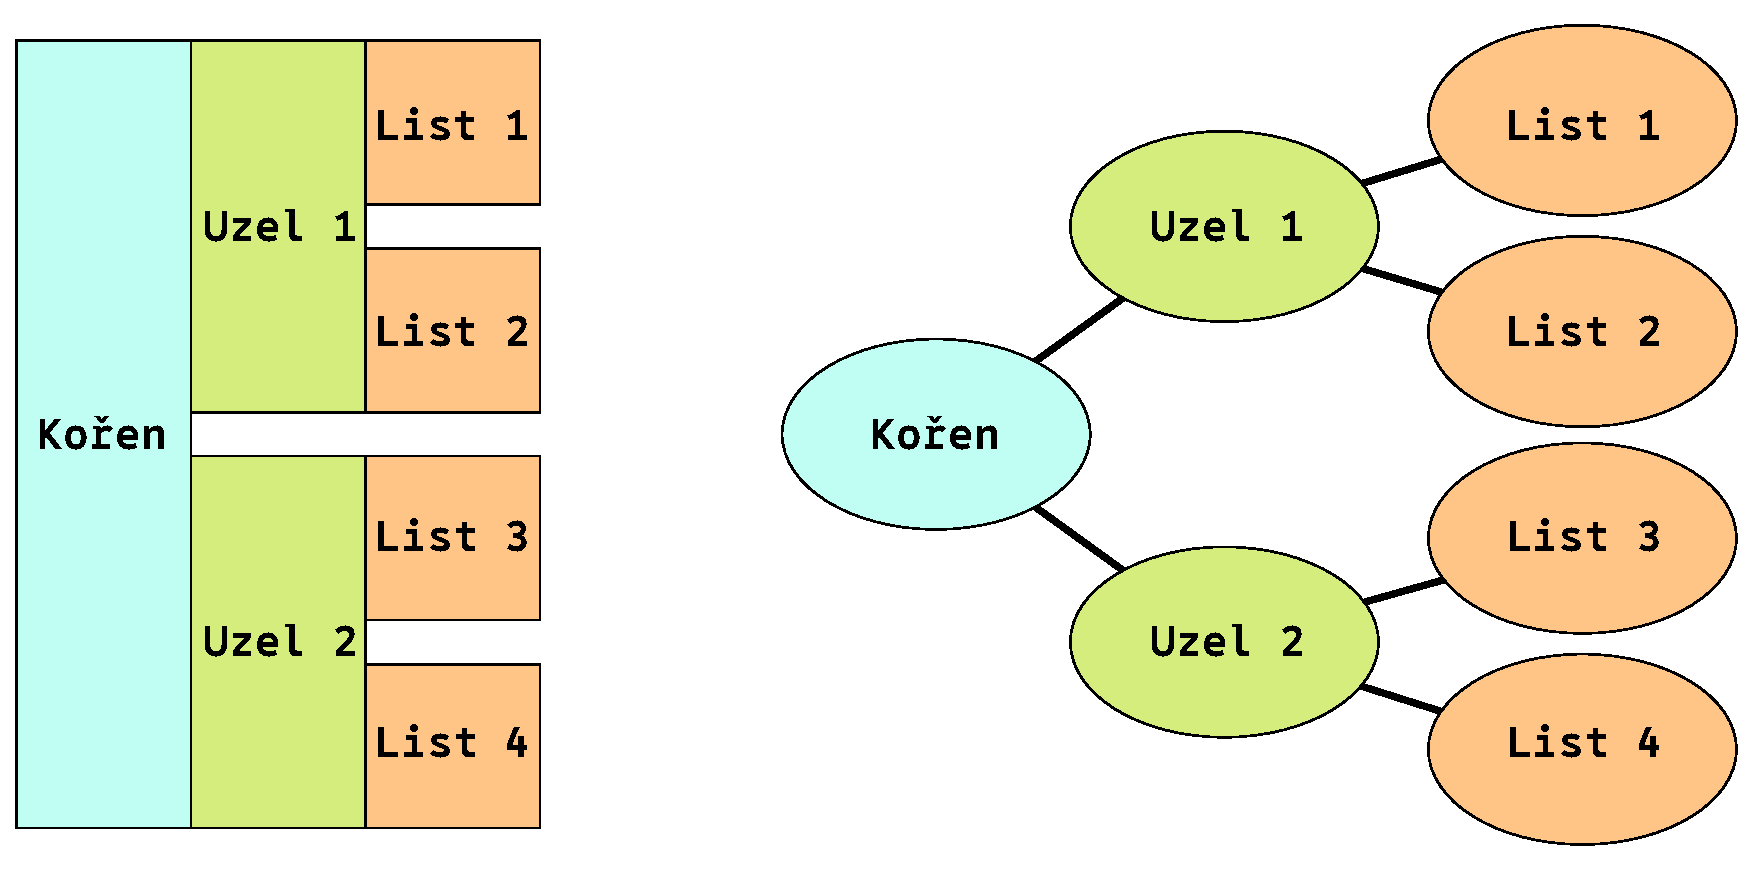
\includegraphics[width=140mm]{img/NUMATV/block-tree.pdf}
        \caption{Blokový strom (vlevo) a klasická grafová reprezentace stromu (vpravo)}
        \label{block-tree}
    \end{figure}
    \item \emph{GL plocha} - kreslící OpenGL plocha používaná KernelSharkem na kreslení CPU grafů a grafů procesů.
    \item \emph{Jádro} - Topologická struktura v Hwlocu obsahující jeden či více procesorů a která je obsažena v NUMA uzlech. Na systémech bez hyperthreadingu je tento termín zaměnitelný s procesorem.
    \item \emph{Logický index} - Index dán části topologie během jejího zkoumání Hwlocem. Společně s typem objektu (PU, jádro, NUMA uzel) pak tvoří unikátní identifikátor komponenty v dané topologii.
    \item \emph{NUMA~TV} - Zkratka pro \uv{NUMA Topology Views}.
    \item \emph{NUMA~TV kontext} - Konfigurační objekt modifikace, který se stará o konfiguraci NUMA~TV pro každý otevřený stream, tj. cestu k souboru topologie, kterou má stream načtenou (pokud vůbec), a který typ pohledu chce stream použít při načtené topologii.
    \item \emph{OS index} - Index přidělen hardwarové komponentě operačním systémem. Nerespektuje topologii a pro vizualizace není moc užitečný. Tyto indexy používá KernelShark pro nápisy u CPU grafů, tj. pokud máme zobrazen graf pro CPU 0, tak \uv{0} je OS indexem daného procesoru.
    \item \emph{Pohled/typ pohledu} - výčtová třída pro vybrání způsobu zobrazení topologie v KernelSharku. NUMA~TV definuje dva pohledy:
    \begin{itemize}
        \item Výchozí pohled, který ignoruje topologii.
        \item \uv{NUMA tree}/stromový pohled, který pro topologii zobrazí topologický strom v topologické ploše.
    \end{itemize} 
    \item \emph{(Procesorový) modul} - Fyzické místo, kde jsou instalovány procesory (dle Hwlocu). Také součást topologie v Hwlocu, může obsahovat jeden i více NUMA uzlů, zároveň jeden modul může být součástí jednoho i více NUMA uzlů.
    \item \emph{PU/procesor} - Hwloc termín pro to samé, co jsou podle KernelSharku CPU. Mohou být seskupeny v jádru, každé jádro má aspoň jeden PU. PU je zkratka z anglického \uv{processing unit}.
    \item \emph{Topologie} - Struktura s detailní organizací paměťových modulů, procesorů, jiných zařízení na stroji/systému a obsahující nějaké dalších informace, jako například jméno stroje či celková paměť. Tuto strukturu dokáže zachytit Hwloc.
    \item \emph{NUMA topologie} - topologie, která se zajímá o NUMA uzly na systému, která jádra jsou k těmto uzlům přidružena/patří těmto uzlům, a které procesory/CPU jsou součástí těchto jader.   
    \item \emph{Topologická plocha} - Qt plocha s topologickým stromem a možnou úlohovou výplní. Je součástí wrapperu topologcké plochy. Lze přímo namapovat na třídu v kódu: \texttt{KsStreamTopoWidget}.
    \item \emph{Topologický strom} - Skupina Qt objektů, které dohromady tvoří blokový strom bez kořene, jehož první vrstvou jsou NUMA uzly, po nich je vrstva jader, které tvoří listy stromu. Topologické stromy jsou vždy součástí topologické plochy. Topologické stromy NUMA~TV vždy vytváří z nějaké zkrácené topologie. Pokud zkrácená topologie nemá více než jeden NUMA uzel, pak se vrstva NUMA uzlů nezobrazuje.
    \item \emph{Úlohová výplň} - Dodatečný prázdný prostor pod topologickým stromem v topologické ploše. Je přítomen pokud KernelShark ukazuje grafy úloh pro nějaký stream.
    \item \emph{Vizualizace topologie} - V NUMA~TV zaměnitelné s topologickým stromem.
    \item \emph{Wrapper topologických ploch/plocha pro zobrazení topologií} - Nalevo od GL plochy, obsahuje topologickou plochu. Existuje z implementačních důvodů.
    \item \emph{Zkrácená topologie} - Reprezentace topologie s pouze nejdůležitějšími částmi pro topologickou vizualizaci od NUMA~TV. Jedná se o třívrstvou strukturu, kde v první vrstvě jsou logické indexy NUMA uzlů, v druhé vrstvě jsou logické indexy jader, ve třetí vrstvě jsou logické indexy procesorů spárovány s OS indexy procesorů.
\end{itemize}

%%%%%%%%%%%%%%%%%%%%%%%%%%%%%%%%%%%%%%%%%%%%%%%%%%%%%%%%%%%%%%%%%%%%%%%
\section{Analýza}
Tato sekce se pokusí zachytit postup, kterým se dostaneme k implementaci řešení. Jedná se o techničtější analýzu než analýza z kapitoly \emph{Obecná analýza a stanovení požadavků}. Zároveň se někdy odkážeme na Couplebreak a části jeho řešení, abychom se zbytečně neopakovali.

\subsection{Hwloc}
Chtěli bychom-li začít se zobrazováním dat topologie od Hwlocu, musíme si nejprve uvědomit, že se jedná o vylepšení, které přidá ke KernelSharku novou závislost, právě Hwloc. Toho jednoduše docílíme editací souborů sestavení pro CMake. Naštěstí pro nás dává dokumentace Hwlocu \cite{Hwloc-Docs} přímý návod, jak dodání závislosti docílit a KernelShark sám už obsahuje jiné závislosti, jejichž instrukcemi sestavení se můžeme inspirovat. Verzi Hwlocu vybereme co možná nejnovější, tj. verzi 2.11.

Na řadu přichází nahrání topologie z XML souboru do datové struktury, se kterou pak může Hwloc pracovat. Dokumentace nám opět pomůže a my můžeme přes Hwloc funkce a makra rovnou načíst XML soubor jako topologii. V té si nejprve získáme všechny OS indexy procesorů/PU a poté si přes každý z nich zjistíme i kterému jádru patří a kterému NUMA uzlu patří. Logické indexy PU, jader a NUMA uzlů si pak uložíme do zkrácené topologie. Abychom neztratili spojení mezi logickými indexy procesorů a jejich OS indexy, uložíme si do zkrácené topologie i OS indexy pro PU. Zkrácenou topologii můžeme implementovat pomocí neseřazených map a indexy můžeme reprezentovat pomocí celých čísel. Zkrácenou topologii použijeme proto, že Hwloc topologie obsahuje informace navíc, které nás u NUMA~TV nezajímají, například uspořádání cache pamětí, nebo jméno stroje, na kterém byla topologie zachycena.

\subsection{Hlášení chyb}

Během nahrávání topologie se může stát nějaká chyba, například nebyl XML soubor ve správném formátu. I ve zbytku modifikace pak mohou nastat chvíle, kdy bude potřeba ošetřit a ohlásit nějakou chybovou či informační situaci. KernelShark sám výjimky nevyhazuje, namísto toho používá zprávy v terminálu nebo informační dialogy. NUMA~TV bude používat návratové kódy a psaní do terminálu pro hlášení nějak zajímavých situací, jako třeba chyb.

\subsection{Konfigurační dialog}
\label{numatv-cfg-subsec}

Poté, co jsme schopni pracovat s Hwlocem a získat si pro nás zajímavá data, se můžeme začít soustředit vytvoření konfigurace NUMA~TV. Začneme GUI pro uživatelskou interakci s konfigurací. Zde si můžeme i rozmyslet, co bude součástí konfigurace, kterou bude tento dialog měnit.

Všimněme si podobností s konfigurací pro Couplebreak \ref{cbreak-cfg-subsec}. I v této modifikaci chceme mít nastavení pro každý stream zvlášť. Můžeme se tedy konfiguračním dialogem Couplebreaku inspirovat a pozměnit jenom to, co pro každý ze streamů konfigurujeme. Naše cíle vyžadují alespoň konfigurovatelnou cestu k XML souboru topologie a typ pohledu, tj. \uv{jak naložit s načtenou topologií}.

Pohledy navíc cíle definují dva, výchozí a stromový. Výchozí pohled už z názvu napovídá, že bude výchozí hodnotou konfigurace pro pohledy. Pohledy můžeme implementovat přes rádiová tlačítka, pak budeme schopni mít vybranou jen jednu možnost pro nějakou skupinu tlačítek.

Výběr XML souboru lze zjednodušit použitím souborového dialogu od Qt a filtrovat pro soubory s příponou \texttt{.xml}. My pak jenom musíme vytvořit nějaké vybírací \texttt{Select} tlačítko, kterým souborový dialog vyvoláme. Ze souborového dialogu pak uložíme cestu k souboru XML jako textový řetězec. Ten pak uživateli zobrazíme, aby bylo jasné, že nějaká topologie byla vybrána. Na vymazání vybrané cesty pak dodáme tlačítko \texttt{Clear}. Výchozí hodnotou cesty k souboru bude přirozeně prázdný text. 

Speciální pozornost dáme tlačítku \texttt{Apply}. To totiž nejenže změny aplikuje, ale před aplikací i zkontroluje některé požadavky, které cíle požadují. Pokud je vybrán stromový pohled, ale nebyl vybrán topologický soubor, pak konfigurace vynutí pohled výchozí, jelikož není co zobrazovat ve stromovém pohledu. Pokud vybereme soubor s topologií o \texttt{N} CPU, ale stream, kterému toto konfigurujeme má \texttt{M} CPU a zároveň \texttt{M} se nerovná \texttt{N}, pak konfigurace opět použije výchozí pohled a uživatel bude o nevhodném souboru topologie informován na chybovém výstupu. Tlačítko \texttt{Cancel} může fungovat jako dřív, tedy prostě dialog zavře bez použití změn.

Tlačítko vyvolávající konfigurační dialog umístíme vedle tlačítka pro konfigurační okénko Couplebreaku, tj. do submenu \texttt{Tools}. Pokud nebude načten žádný stream, toto tlačítko ukáže informační okénko se zprávou, že pro konfiguraci modifikace je nutné mít otevřen alespoň jeden stream.

\subsection{Konfigurace NUMA~TV}

V předchozí podsekci jsme si už trochu seznámili s tím, jak se bude konfigurace chovat, hlavně z grafického pohledu. Nyní se zamyslíme nad tím, jak by se měla chovat mimo grafické prostředí.

Nejprve se zamyslíme nad tím, jak reprezentovat pohledy. My implementujeme jenom stromový pohled na NUMA topologii, ale teoreticky jich může být více, například pohled na procesorové moduly. Proto pohledy implementujeme jako výčtový typ. Tak se omezíme jen na nějakou konečnou množinu hodnot a budeme mít kódu zřetelněji popsané speciální číselné hodnoty.

Dokud uživatel nezmění konfiguraci v dialogu z výchozích hodnot, pak modifikace nebude ukládat žádnou konfiguraci pro stream, jelikož by to bylo zbytečné. Pokud ale uživatel vybere validní XML soubor s topologií, pak se situace mění. Aplikace konfigurace pak donutí NUMA~TV vytvořit novou konfiguraci pro stream, včetně interpretace topologického XML souboru Hwlocem. Po ní nám zbyde zkrácená topologie, kterou také uložíme do konfigurace pro stream. Z toho nám vyplývá, že datová struktura konfigurace NUMA~TV pro nějaký stream bude obsahovat prvky pro uložení cesty k XML souboru, uložení typu pohledu a uložení zkrácené topologie.

Pokud uživatel vymaže v konfiguračním dialogu cestu k topologickému souboru, pak není konfigurace pro stream potřeba. Pro nás to znamená návrat k výchozím hodnotám konfigurace (i kdyby byl vybrán stromový pohled, tak bez cesty k souboru topologie toto NUMA~TV změní na výchozí pohled). Abychom zbytečně neukládali nepotřebnou konfiguraci, tak ji v této situaci smažeme.

Dalším problémem, co vyřešíme, je aktualizace topologie. Ta se stane, když uživatel změní cestu k topologickému souboru a nebo změní typ pohledu v konfiguračním dialogu a změny aplikuje. Pokud změní cestu, pak lze považovat starou konfiguraci topologie za zbytečnou a tak ji smažeme. Můžeme ji pak kompletně nahradit novou konfigurací. Pokud se změnil jen pohled, pak změníme jen ten. V každém případě ale požádáme  NUMA~TV o překreslení topologických vizualizací (vizualizační část je popsána v nižší sekci \ref{numatv-grt}). Pokud je topologie nějak nevalidní (případy popsány v sekci o konfiguračním dialogu výše \ref{numatv-cfg-subsec}), pak návratovým kódem rozhodneme, jak se má KernelShark zachovat tj. jestli má do terminálu napsat nějakou chybovou zprávu.

Pokud uživatel nepřidá nový otevřený stream, ale místo toho otevře pouze jeden nový (tj. použije tlačítko \texttt{Open Trace File} namísto tlačítka \texttt{Append Trace File}), konfigurace všech streamů zahodíme.

Nakonec, namísto ukládání konfigurací ke každému streamu zvlášť si pořídíme manažera konfigurací, tzv. NUMA~TV (konfigurační) kontext. Ten si bude pro každý stream pamatovat jeho specifickou konfiguraci. Krom toho bude mít i API pro přidávání, odebírání, a aktualizaci konfigurací pro každý stream. Jelikož mezi streamy mohou být \uv{díry}, tj. ne každý stream musí mít aktivní NUMA~TV konfiguraci, bude nejlepší i toto vyřešit mapou, klidně i nesetříděnou, jelikož je zbytečné mít konfigurace uspořádané. Kontext bude mít i možnost dát nějakému žadateli observer ukazatel na uloženou konfiguraci a ptát se, zdali konfigurace existuje. Funkci k získání observeru i explicitně pojmenujeme tak, že bude jasné, že tento ukazatel nemá být jakkoliv použit k řízení životnosti. Navíc bude ukazatel brát ukazovanou hodnotu jako konstantní, tj. neměnitelnou, měnit konfiguraci bude schopen pouze NUMA~TV kontext jakožto její vlastník.

\subsection{Grafická reprezentace topologie}
\label{numatv-grt}
Vyřešili jsme konfiguraci i jak ji může uživatel měnit. Zatím ale vůbec nemá efekt. Posuňme se tak k vizualizaci topologie.

\subsubsection{Topologický strom}
Nejprve si upřesníme, jak budeme topologii vizualizovat. Cíle nám již celkem podrobně předdefinovali, že se má jednat o strom s popisky prvků, ve kterém budou vrcholy jádra a NUMA uzly, a pokud je NUMA uzlů na systému detekováno více než jeden. My už jen dotáhneme, jak přesně tato vizualizace bude vypadat. Namísto stromů stvořených z uzlů a hran použijeme blokový strom, viz obrázek \ref{block-tree}. Tím nebudeme muset řešit kreslení hran, jen pozice bloků a mezery mezi nimi. Topologie má v Hwlocu stromovou strukturu, jejímž kořenem je stroj, na kterém byla zachycena. Stroj pro nás není moc důležitý (spojili bychom ho s nějakým streamem), ve stromu tedy nebude. S šikovným umístěním vizualizace v KernelSharku bychom ani nemuseli kreslit vrcholy pro procesory. Jelikož nechceme kreslit pouze jeden NUMA uzel, pak topologický strom bude ve skutečnosti vždy lesem - buď budou jednotlivé stromy zakořeněny ve dvou či více NUMA uzlech, které nebudou spojeny vrcholem pro stroj, nebo zobrazíme jenom několik vrcholů pro jádra. Implicitně ale všechny vrcholy v tomto lese sdílí jediného předka, stroj - my jsme jen odsekli nepotřebné části.

Barvy máme také předdefinovány. Barvu procesoru získáme z KernelSharku, který už takové generuje. S dodatečným vylepšením \emph{Get Colors} pak můžeme i jednoduše tyto barvy získat.

Popisky vrcholů ve stromu budou jednoduché zkratky, aby se do bloku vešel text. Psát je budeme jako ostatní text v KernelSharku, tj. nebudeme je nijak rotovat, či zvětšovat - tím neztratíme čitelnost. Navíc dodáme plovoucí vysvětlivky (anglicky \uv{tooltip}), které se zobrazí po přejetí myši přes blok, čímž usnadníme čitelnost a odstraníme nutnost vždy zjišťovat významy zkratek v uživatelské dokumentaci. Za zkratky a někam do vysvětlivky přidáme logický index dané komponenty topologie. Popisky budou vždy v centru bloku. Pokud bude strom obsahovat NUMA uzly, tak do popisku i vysvětlivky pro vrchol jádra přidáme prefix pro určení NUMA uzlu, kterému jádro patří. Pokud nebudeme schopni vidět blok pro NUMA uzel a nebude se nám chtít čekat, budeme tak schopni ihned určit NUMA uzel nějakého jádra. Jelikož bloky mohou mít různé barvy, tak ještě zajistíme, že dle tmavosti dané barvy budeme používat buď černý, nebo bílý text.

Hodnoty mezer mezi bloky můžeme získat z GL plochy KernelSharku, která je má uložené a používá je při kreslení všech grafů.

Se stromem nebudeme schopni nijak interagovat, kromě zobrazení vysvětlivek.

\subsubsection{Místo pro topologický strom}
Topologický strom máme navržen. Nyní přichází otázka, kam jej umístit. Už jsme zmínili \uv{šikovné umístění}, díky kterému nebudeme muset ani zobrazovat bloky pro procesory. Ještě předtím se ale krátce zamysleme, kde by viditelný topologický strom byl nejpříjemnější. Umístění vlevo, vpravo, nebo pod seznamem událostí nejsou vhodná. Topologický strom nemá se seznamem nic společného. Umístění mezi seznamem a grafem trasování je také nevhodné, jelikož by hlavní okno muselo být vertikálně rozděleno ještě více než doposud. Protože obrazovky jsou často orientovány na šířku, tak bychom si zmenšili jak seznam, tak graf trasování, což by zhoršilo příjemnost čtení v hlavním okně. Stejný argument pak platí pro umístění nad graf trasování. Cíle nám ale udávají umístění v hlavním okně. Pak bychom mohli vizualizaci topologie umístit nalevo nebo napravo od grafu trasování. Ani jedno z umístění není špatné, jak vpravo, tak vlevo bychom mohli topologický strom zobrazit tak, aby se napojoval na grafy CPU, kterými bychom reprezentovali procesory v topologii. Umístění vlevo má ale jednu výhodu. Nápisy grafů v KernelSharku jsou nalevo od samotného grafu a pokud i my umístíme strom vlevo od grafu trasování, pak budou nápisy pro topologický strom blízko nápisů pro grafy, což je vizuálně jednotnější, než umístění vpravo. Oči uživatele nemusí běhat z jedné strany okna na druhou, mohou se pohybovat jen na levé straně, což bude pro uživatele příjemnější.

Vytvoříme tedy místo pro topologický strom, nazveme jej topologická plocha. Růst stromu orientujeme doprava, tj. nejprve zobrazíme NUMA uzly, pak vlevo jádra a po nich budou v grafu trasování následovat CPU. Jelikož procesy nemají na topologii vliv, budou nás zajímat jen CPU grafy. KernelShark nejprve vždy zobrazuje CPU grafy a až poté grafy úloh. Topologická plocha tak bude začínat topologickým stromem a pod něj vloží úlohovou výplň, jsou-li ve streamu, pro který byl tento strom zobrazen, přítomny nějaké grafy úloh. Výšky bloků topologického stromu pak budou odvozeny od výšek grafů v GL ploše a mezerami mezi nimi. Abychom mohli blokový strom jednodušeji nakreslit, přeuspořádáme CPU grafy tak, aby se směrem dolů zvedaly logické indexy, nikoli OS indexy, jak to dělal KernelShark doposud. K vytvoření topologického stromu v topologické ploše pak jednoduše pro stream, který vlastní topologickou plochu, získáme konfiguraci z NUMA~TV kontextu a pokud chceme stromový pohled, pak použijeme zkrácenou topologii ke konstrukci. Pokud žádný stream nechce zobrazit topologii (není načtená, nebo je nakonfigurován výchozí pohled), pak nebudeme strom vytvářet a topologická plocha bude prázdná.

Kdy budeme kreslit topologické stromy a upravovat úlohové výplně? K tomu vyžijeme dvě \uv{redraw} funkce - \texttt{cpReDraw} a \texttt{taskReDraw}, obě specifické pro nějaký stream. První se volá vždy, když mají být z nějakého důvodu překresleny CPU grafy, například pokud chceme jeden z nich schovat. Druhá z funkcí má podobný úkol, ale týká se grafů procesů. Obě funkce upravíme - \texttt{taskReDraw} bude měnit velikost úlohové výplně v topologické ploše upravovaného streamu, pokud se počet grafů procesů změní; \texttt{cpuReDraw} bude mít možnost měnit topologický strom za jiný, měnit uspořádání CPU grafů a nakonec také upraví úlohovou plochu, resp. její umístění. Obě tyto funkce zavoláme i při úspěšné změně konfigurace, abychom její efekt viděli ihned. Přirozeně pak bude možné i měnit prvky topologické plochy i při jiných změnách grafů, jako právě při jejich schovávání či zviditelnění.

Každý stream bude mít vlastní topologickou plochu, jelikož každý stream má vlastní CPU grafy. Nyní tedy musíme zobrazit několik topologických ploch, pokud máme ve streamu otevřeno více streamů. Pro seskupení topologických ploch vytvoříme jiný grafický objekt, wrapper topologických ploch. Wrapper bude přímým sousedem grafu trasování a topologické plochy v něm budou uspořádány odshora dolů, s mezerami na hranicích streamů. Synchronizujeme i rolování v grafu trasování s rolováním ve wrapperu, aby naše stromy byly neustále napojeny na CPU grafy. Wrapper a jemu podřízené prvky nebudou vůbec zobrazeny, pokud každý stream chce zobrazit svou topologii výchozím pohledem (či nemá načtenou topologii).

Zatím jsme se nebavili o velikosti místa pro topologické plochy (resp. jejich wrapper, plochy mohou svou velikost a velikost svých prvků odvozovat od něj). Výška wrapperu bude stejná jako výška grafu trasování. Bez exaktních výzkumů optimálního poměru šířky topologického stromu a grafu trasování ale můžeme odhadnout, že pokud graf trasování dříve zabíral 100 \% svého vymezené šířky v hlavním okně, tak by asi neuškodilo zabrat pětinu této šířky. Tak bude graf trasování stále hlavním prvkem hlavního okna vedle seznamu událostí a topologie bude mít dost prostoru na zobrazení topologického stromu.

\subsubsection{Skrývající tlačítko}
Cíle nám ještě určují, že máme být schopni místo s vizualizací topologie skrývat. K tomu vytvoříme jednoduché tlačítko, které umístíme nalevo od wrapperu topologických ploch, abychom neoddělovali topologický strom od CPU grafů. Na kliknutí myši toto tlačítko pomocí Qt skryje wrapper a graf trasování se natáhne až k tlačítku. Na další kliknutí se opět zobrazí wrapper a graf trasování se zkrátí. Tlačítko bychom měli nějak pěkně stylizovat, aby bylo jasné, k čemu slouží. To jde vcelku jednoduše přidáním symbolů \texttt{<} a \texttt{>}, které budeme měnit podle stavu viditelnosti wrapperu. Pro zvýraznění tlačítka nějakou nerušivou barvou použijeme zelenou. Stejně jako wrapper, toto tlačítko nebude vůbec viditelné, pokud každý stream má v konfiguraci vybrán výchozí pohled (tedy buď topologii zobrazit nechce, nebo žádnou topologii nemá).

\subsection{Relace}
Relace implementujeme mnohem snadněji než u Couplebreaku. NUMA~TV uloží pod identifikátor streamu vybraný typ pohledu a cestu k XML souboru (nebo žádnou cestu neuloží v případě nevybraného souboru v konfiguraci). Inspirovat se můžeme ostatním kódem pro ukládání relace, například pro ukládání Markerů A a B. A stejně se inspirujeme i pro načítání NUMA~TV z relačního souboru.

Nyní zbývá vybrat momenty, kdy ukládat NUMA~TV a hlavně kdy relační data pro modifikaci načítat. Nelze načítat kdykoliv, jelikož bychom jinak nezastihli vykreslení CPU grafů, tedy i jejich možnou reorganizaci, což by vizualizaci úplně pokazilo. Načítat relační data proto budeme před načtením grafu, abychom vykreslení CPU stihli. Ukládání není závislé na pořadí ukládání ostatních částí relace, ale kvůli symetrii s načítáním jej zařadíme před ukládání grafů.

\subsection{Zařazení mezi existující kód}
Nakonec musíme zjistit, kde budou části NUMA~TV žít. Jelikož jsme hluboce spjati s grafem trasování, nejlepším místem pro konfigurační kontext i topologické plochy bude právě třída pro něj. V ní máme jednoduchý přístup k \uv{redraw} funkcím, jelikož jsou její součástí a pokud rozšíříme existující API, můžeme dovolit jiným částem KernelSharku komunikovat s NUMA~TV, pokud mají ke grafu trasování přístup. Konfigurační dialog pak může být samostatná třída vyvolávaná hlavním oknem při stisknutí příslušného tlačítka. Hlavní okno pak bude mít na starosti komunikaci mezi dialogem a konfiguračním kontextem. Hlavní okno také určuje pořadí ukládání relačních dat, upravovat toto pořadí musíme v něm.

%----------------------------------------------------------------------

\subsection{Zamítnutá alternativní řešení}
Tato část je souhrnem několika nápadů, které se objevily během vymýšlení řešení či přímo během implementace, ale byly nakonec zavrženy z různých důvodů. Představen bude jak návrh řešení, tak důvod zamítnutí.

\subsubsection*{Konfigurační kontext jako singleton}
Během prvotních návrhů byl NUMA~TV kontext původně singletonem. Důvod byl jednoduchý - je nutné vždy znát konfiguraci a chceme vždy jen jednu. A dlouhou dobu během implementace se s kontextem opravdu pracovalo, jako se singletonem. Nicméně KernelShark singletony nepoužívá a skrytých závislostí přibývalo. Proto bylo nakonec rozhodnuto o refaktorizaci kontextu do součásti grafu trasování, kde nakonec žily i topologické plochy.

\subsubsection*{Kreslení stromu do GL plochy}
Jedním z prvních návrhů pro umístění topologického stromu byla GL plocha v grafu trasování. Cílem bylo posunout všechny ostatní kreslené objekty a vložit strom topologie nalevo. Čím více se ale zjistilo o práci s touto plochou, tím spíše se ukázalo, že toto byl špatný nápad. Pro úpravu v této ploše bylo odhadnuto enormní množství úprav, oproti prvotnímu nápadu \uv{prostě vše posunout}, na který neměla plocha dostatečně mocné API. Návrh byl proto zamítnut.

\subsubsection*{Graf vytvořen přes QTreeWidget}
Namísto blokového stromu, který lze vytvořit i jen pomocí vertikálních a horizontálních rozložení spolu s textovými krabičkami, byl zvážen i \texttt{QTreeWidget}, který KernelShark používá v okénku jednoduchých filtrů událostí. Nicméně interakce a rozložení této předdefinované třídy bez úprav nebyly po zamítnutí možnosti stromy skládat pro NUMA~TV užitečné a tak byl návrh zahozen.

%%%%%%%%%%%%%%%%%%%%%%%%%%%%%%%%%%%%%%%%%%%%%%%%%%%%%%%%%%%%%%%%%%%%%%%
\section{Vývojová dokumentace}
Tato sekce chce čtenáři načrtnout strukturu modifikace, podle které se lze v modifikaci orientovat. Také dodá krátký návod pro vývojáře, kteří by chtěli s NUMA~TV pracovat ve svých pluginech či změnách pro KernelShark.

NUMA~TV představuje úplně novou funkcionalitu a dá se označit za nový modul pro KernelShark, který je úzce spojen s modulem hlavního okna, jelikož využívá data a funkce grafu trasování a jeho GL plochy. Je také vázán na modul relací, ovšem slaběji, pouze skrze API. 

\subsubsection*{Názvy}
Stejně jako u Couplebreaku, i zde zmíníme názvy pro nové prvky v kódu modifikace. Zde neexistuje pouze jedna posloupnost znaků, kterými můžeme nový kód identifikovat. Namísto toho jsou všechny novinky pojmenovány tak, že někde v jejich jméně je buď \texttt{numatv}, \texttt{topology}, nebo zkratkovitě \texttt{topo}, tyto tři označení mohou být i psána velkými písmeny. Tak je tomu v nových API, ale i v čistě implementačních funkcích, pokud nebyla značka v ohraničujícím komentáři sama ohraničena uvozovkami (viz vysvětlení ohraničujících komentářů \ref{comment-style}).

\subsection{Struktura modifikace}
Modifikaci rozdělíme na moduly. Pro detailnější informace a implementační detaily je doporučeno prohlédnout si samotný kód a technickou Doxygen dokumentaci KernelSharku, jejíž novou součástí jsou i části o modifikaci.

Ke každému modulu připíšeme i soubory, ve kterých je modul implementován, a prvky modulu jako veřejné funkce, či třídy. Prvky mimo hlavičkové soubory, nebo označeny za privátní pro třídu jsou brány jako implementační detaily a nebudou zde popsány (lze je najít uvnitř souborů modulu).

V kódu modifikace používá značku \texttt{NUMA~TV} v ohraničeních změn.

\subsubsection*{Konfigurace}
Modul řeší konfiguraci NUMA~TV pro každý stream, včetně konfiguračního kontextu, přes který je řízen vznik, změny a zánik konfigurací. Součástí modulu je i okénko pro konfigurační dialog.

\begin{itemize}
    \item \textbf{Soubory:} KsWidgetsLib.hpp/cpp, KsMainWindow.hpp/cpp, KsNUMATopologyViews.hpp/cpp, KsTraceGraph.hpp/cpp
    \item \textbf{Třídy:}
    \begin{itemize}
        \item \emph{KsNUMATVDialog} - grafické okno, konfigurační dialog pro NUMA~TV.
        \item \emph{KsTopoViewsContext} - NUMA~TV kontext, tj. manažer konfgurací pro streamy.
        \item \emph{StreamNUMATopologyConfig} - konfigurace NUMA~TV pro nějaký jeden stream.
        \item \emph{TopoViewType} - výčtová třída pro typy pohledů v NUMA~TV.
    \end{itemize}
    \item \textbf{Typové aliasy:}
    \begin{itemize}
        \item \emph{ViewTopologyPair} - pár reprezentující pohled a cestu k topologickému souboru.
        \item \emph{TopoPUIds} - pro mapování logických indexů procesorů na jejich OS indexy. Součást zkrácené topologie.
        \item \emph{TopoCorePU} - pro mapování logických indexů jader na TopoPUIds. Součást zkrácené topologie.
        \item \emph{TopoNodeCorePU} - pro mapování logických indexů NUMA uzlů na TopoCorePU. Představuje zkrácenou topologii.
    \end{itemize}
    \item \textbf{Nové API} třídy \emph{KsTraceGraph}: nová funkce \emph{getNUMATVContext}, získá referenci na NUMA~TV kontext s konfiguracemi streamů.
\end{itemize}

Tento modul je také důvodem změny souboru \emph{CMakeLists.txt} v adresáři zdrojového kódu KernelSharku, jelikož soubory jej obsahující jsou nové.

\subsubsection*{Propojení s Hwlocem}
Mini-modul se stará zejména o vytváření zkrácených topologií z dat Hwlocu. Úzce spolupracuje s modulem Konfigurace. Je vydělen z modulu Konfigurace kvůli specificitě své práce. Modul řeší čistě implementaci a nelze s ním komunikovat skrze veřejná rozhraní.

\begin{itemize}
    \item \textbf{Soubor:} KsNUMATopologyViews.cpp
\end{itemize}

\subsubsection*{API zkrácených topologií}
Modul je souhrnem pár funkcí, které mohou se zkrácenou topologií nějak pracovat, například z ní vypočítat nějaké hodnoty.

\begin{itemize}
    \item \textbf{Soubory:} KsNUMATopologyViews.hpp/cpp
    \item \textbf{Typové aliasy:}
    \begin{itemize}
        \item \emph{TopoPUIds} - pro mapování logických indexů procesorů na jejich OS indexy. Součást zkrácené topologie.
        \item \emph{TopoCorePU} - pro mapování logických indexů jader na TopoPUIds. Součást zkrácené topologie.
        \item \emph{TopoNodeCorePU} - pro mapování logických indexů NUMA uzlů na TopoCorePU. Představuje zkrácenou topologii.
    \end{itemize}
    \item \textbf{Globální funkce:}
    \begin{itemize}
        \item \emph{numatv\_count\_PUs} - spočítá, kolik PU, tj. procesorů, je ve zkrácené topologii.
        \item \emph{numatv\_count\_cores} - spočítá, kolik jader je ve zkrácené topologii.
        \item \emph{numatv\_filter\_by\_PUs} - vrátí zkrácenou topologii, jejímiž prvky jsou pouze procesory specifikované v argumentu a prvky topologie procesory obsahující.
    \end{itemize}
\end{itemize}

\subsubsection*{Vizualizace}
Tento modul řeší grafické znázornění zkrácené topologie, umístění topologických stromů v hlavním okně a jejich správné napojení na CPU grafy. Součástí je i skrývající tlačítko wrapperu topologických ploch.

\begin{itemize}
    \item \textbf{Soubory:} KsStreamNUMATopology.hpp/cpp, KsMainWindow.cpp, KsTraceGraph.hpp/cpp
    \item \textbf{Třídy:}
    \begin{itemize}
        \item \emph{KsTopologyScrollArea} - upravuje implementaci zpracování rolování kolečkem na myši resp. tyto události ignoruje.
        \item \emph{KsStreamNUMATopology} - reprezentuje topologickou plochu a topologický strom.
    \end{itemize}
    \item \textbf{Nové API} třídy \emph{KsTraceGraph}:
    \begin{itemize}
        \item \emph{numatvClearTopologyWidgets} - funkce zničí topologické plochy a topologické stromy v nich.
        \item \emph{numatvHideTopologyWidget} - funkce dle argumentu nastaví viditelnost wrapperu topologických ploch.
    \end{itemize}
\end{itemize}

\subsubsection*{Relace}
Modul se stará o integraci NUMA~TV do relací KernelSharku, tj. o ukládání a načítání hodnot pro konfigurace této modifikace.

\begin{itemize}
    \item \textbf{Soubory:} KsSession.cpp/hpp, KsMainWindow.cpp
    \item \textbf{Nové API} třídy \emph{KsSession}:
    \begin{itemize}
        \item \emph{saveTopology} - funkce uloží data NUMA~TV konfigurací do relačního souboru.
        \item \emph{loadTopology} - funkce načte NUMA~TV konfigurace z dat v relačním souboru.
    \end{itemize}
\end{itemize}

\subsection{Úpravy mimo logiku modifikace}

\subsubsection*{Funkce v \emph{KsPlot} jmenném prostoru}
Přidané funkce pomáhají hlavně s rozhodováním mezi černou a bílou barvou dle intenzity nějaké barvy. Obě použity v modulu \emph{Vizualizace}. Přidané funkce jsou následující:
\begin{itemize}
    \item \emph{blackOrWhite} - rozhodne, zdali je pro nějakou intenzitu barvy více výrazná černá nebo bílá barva.
    \item \emph{getColorIntensity} - spočítá intenzitu barvy.
\end{itemize}

\subsubsection*{Úpravy instrukcí sestavení}
Následující soubory byly přidány, aby bylo možné NUMA~TV připojit ke KernelSharku a přidat Hwloc jako závislost:
\begin{itemize}
    \item \emph{(build/)FindHwloc.cmake} - nový soubor s detailními instrukcemi pro hledání Hwlocu na systému. 
    \item \emph{CMakeLists.txt} - do tohoto souboru pro sestavení byly přidány instrukce k nalezení Hwlocu, tj. pro vynucení závislosti KernelSharku na Hwlocu. (Tento soubor je v kořenovém adresáři pro KernelShark, \texttt{KS\_fork}.)
    \item \emph{(src/)CMakeLists.txt} - zde byly nové soubory NUMA~TV přidány do kompilace GUI knihovny pro KernelShark. K této knihovně zde byl připojen i Hwloc. (Tento soubor je v adresáři pro zdrojový kód KernelSharku, \texttt{KS\_fork/src}.)
\end{itemize}

\subsection{Vyvíjení pro KernelShark s NUMA~TV}
NUMA~TV jako nový modul KernelSharku se snaží být oddělen od ostatních modulů, kromě modulu hlavního okna a relací. Pokud tedy vyvíjíme pro KernelShark a neřešíme změny těchto modulů, lze NUMA~TV kompletně ignorovat. Modul navíc neřeší trasovací data, takže jakékoli změny dat netýkající se identifikace CPU, jako například změny v datech od modifikace Couplebreak, bude NUMA~TV ignorovat.

Pluginy s modulem nijak přímo spolupracovat nemohou, ale pokud získají ukazatel na hlavní okno a dostanou se k objektu grafu trasování, pak je možné použít některou z funkcí přidanou k tomuto objektu, jako třeba získání NUMA~TV kontextu. Za použití funkcí v kódu pak samozřejmě odpovídá vývojář a musí si dát pozor, aby implementaci nerozbil.

Při vývoji jak pluginu, tak dalšího kódu pro KernelShark je samozřejmě také možné použít nové veřejné funkce a třídy od NUMA~TV, pokud si vložíme správné hlavičkové soubory přes \texttt{\#include}. Chceme-li například vytvořit nějakou rozšířenou konfiguraci NUMA~TV, pak budeme nejspíš používat či měnit třídu \texttt{StreamNUMATopologyConfig}. 

%%%%%%%%%%%%%%%%%%%%%%%%%%%%%%%%%%%%%%%%%%%%%%%%%%%%%%%%%%%%%%%%%%%%%%%
\section{Uživatelská dokumentace}

\subsection{Stav při otevření KernelSharku}

NUMA~TV není (skoro) nijak pozorovatelná při spuštění KernelSharku. Zůstává skryta i při načtení trasovacích dat, nebo i pokud načítáme relaci, kde konfigurace NUMA~TV nebyla uložena, nebo jsou pro všechny streamy v relaci nastaveny výchozí pohledy (tj. typy zobrazení topologie, přičemž výchozí nezobrazují topologii). Aby měla modifikace nějaký viditelný vliv, musíme ji k tomu nejprve nakonfigurovat. Obrázek \ref{numatv-2} zobrazuje relaci KernelSharku bez aktivní NUMA~TV.

\begin{figure}[p]\centering
    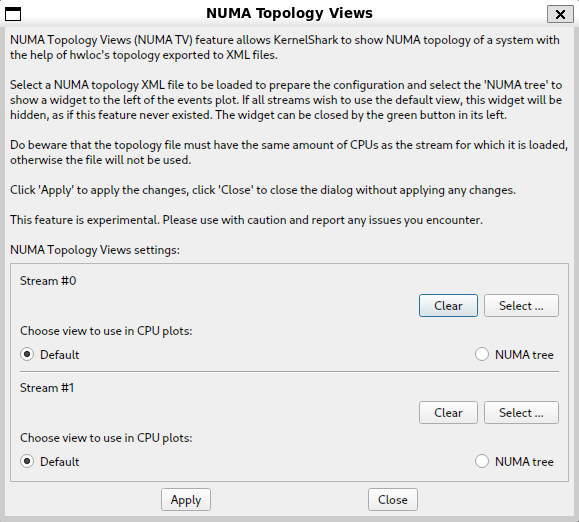
\includegraphics[width=140mm]{img/NUMATV/numatv-2}
    \caption{Neaktivní NUMA~TV v KernelSharku není vizuálně přítomna}
    \label{numatv-2}
\end{figure}

\subsection{Konfigurace}

Abychom mohli NUMA~TV nakonfigurovat, bylo do submenu \texttt{Tools} v hlavním menu přidáno tlačítko \texttt{NUMA Topology Views} na zobrazení konfiguračního dialogu. Pokud nebyl zatím načten žádný stream, zobrazí se vyskakovací okénko, které na tento fakt upozorní. Konfigurační dialog nebude v této situaci zobrazen.

Pokud máme načtený alespoň jeden stream, pak se konfigrační dialog po stisknutí tlačítka zobrazí. Dialog obsahuje vysvětlení modifikace v horní části, pak rolovatelnou plochu s konfiguracemi NUMA~TV pro každý otevřený stream a nakonec dvě tlačítka, \uv{Apply} a \uv{Close}. Tlačítko \uv{Close} zavře konfigurační dialog a neuloží provedené změny. Tlačítko \uv{Apply} se při stisknutí pokusí uložit provedené změny do konfigurací pro každý změněný stream, případně vytvoří konfigurace nové.

Každý stream má pak vůči NUMA~TV dva prvky ke konfiguraci, tj. cestu k XML souboru s topologií od Hwlocu a pohled, který má KernelShark pro danou topologii použít. V současnosti existují dva podporované pohledy, pohled výchozí a pohled stromový (v dialogu označeny jako \uv{Default} pro výchozí pohled a \uv{NUMA tree} pro pohled stromový).

K výběru topologického souboru slouží tlačítka \uv{Clear} a \uv{Select ...}. Tlačítko \uv{Clear} nastaví cestu na prázdný text. Tlačítko \uv{Select ...} zobrazí dialog pro výběr XML souborů na systému. Souborový dialog vždy začíná v domovském adresáři uživatele (standardně adresář \texttt{/home/[USER]}, kde \texttt{[USER]} je jméno uživatele), ale pokud je již vybrán nějaký topologický soubor, tak dialog začne v adresáři s tímto souborem. Vybrané XML soubory nemusí být validní pro daný stream, v tom případě se toto zjistí při pokusu aplikovat změny konfigurace, pokus selže, tj. konfigurace bude stejná jako před pokusem o změnu, a uživatel o této situaci bude informován v terminálu. Nevalidní soubory buď vůbec nejsou interpretovatelné Hwlocem, nebo obsahují odlišný počet procesorů než stream. Pokud nemáme vybranou cestu k XML souboru, nebo jsme ji smazali, pak aplikace změn NUMA~TV konfiguraci pro daný stream nastaví na výchozí hodnoty, tj. prázdnou cestu a výchozí pohled (i kdyby byl předtím vybrán stromový pohled).

Výchozí pohled značí výchozí chování KernelSharku, což je ignorování jakýchkoli topologických informací. Stromový pohled zobrazí NUMA topologii systému zachycenou ve vybraném XML souboru konfigurace streamu jako strom (o vizualizaci později).

Opětovným otevřením konfiguračního dialogu uvidíme hodnoty současných konfigurací streamů. To znamená, že kdybychom změnili v konfiguračním dialogu nějaké hodnoty, ale změny neaplikovali, tak jsou tyto změny ztraceny právě proto, že konfigurační dialog vždy při otevření zobrazí aktuální použité hodnoty konfigurací.

\subsection{GUI}

\subsubsection{Kde jsou zobrazeny topologie}

Obrázek \ref{numatv-3} zobrazuje relaci KernelSharku s jedním streamem, který používá stromový pohled na svou NUMA topologii.

\begin{figure}[p]\centering
    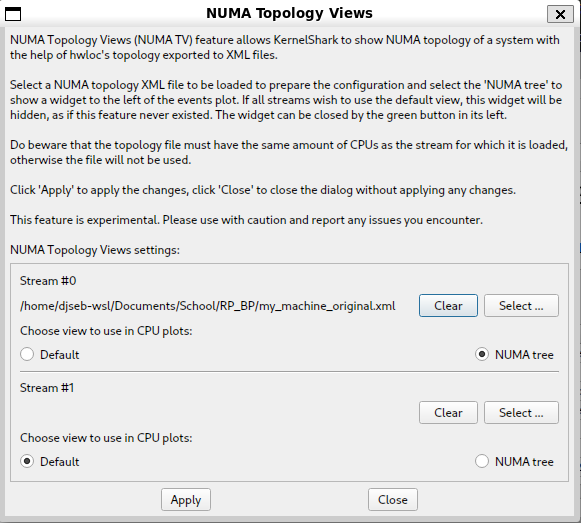
\includegraphics[width=140mm]{img/NUMATV/numatv-3}
    \caption{Aktivní NUMA~TV pro jeden otevřený stream}
    \label{numatv-3}
\end{figure}

Plocha pro zobrazení topologií je zobrazena vždy, když alespoň jeden stream žádá o jiný než výchozí pohled ve své konfiguraci. Pokud stream zobrazuje alespoň některé ze svých CPU grafů, pak plocha pro zobrazení topologií zobrazuje topologický strom pro tento stream (viz níže). Pokud je plocha pro zobrazení topologií zobrazená, ale stream chce použít výchozí pohled, pak se v ploše nezobrazí pro tento stream nic, i kdyby nějaké CPU grafy ukazoval.

Aby topologické stromy zůstaly napojeny na CPU grafy v GL ploše i pokud jsme se v ní posunuli níže, tak při rolování v GL ploše se posouvá i obsah plochy pro zobrazení topologií. V ní samotné nijak rolovat nelze. Pokud je hlavní okno KernelSharku příliš úzké, zobrazí se pro tuto plochu horizontální rolovací posuvník. Ovšem v takové situaci je spíše doporučeno rozšířit KernelShark.

Pokud je plocha pro zobrazení topologií viditelná, je viditelné i skrývající zelené tlačítko nalevo od této plochy, kterým můžeme plochu schovat a nebo znovu zviditelnit. Text tlačítka je buď \uv{<} pro schování, nebo \uv{>} pro zobrazení plochy. Tlačítko v akci můžeme vidět na obrázcích \ref{numatv-5} a \ref{numatv-6}.

\begin{figure}[p]\centering
    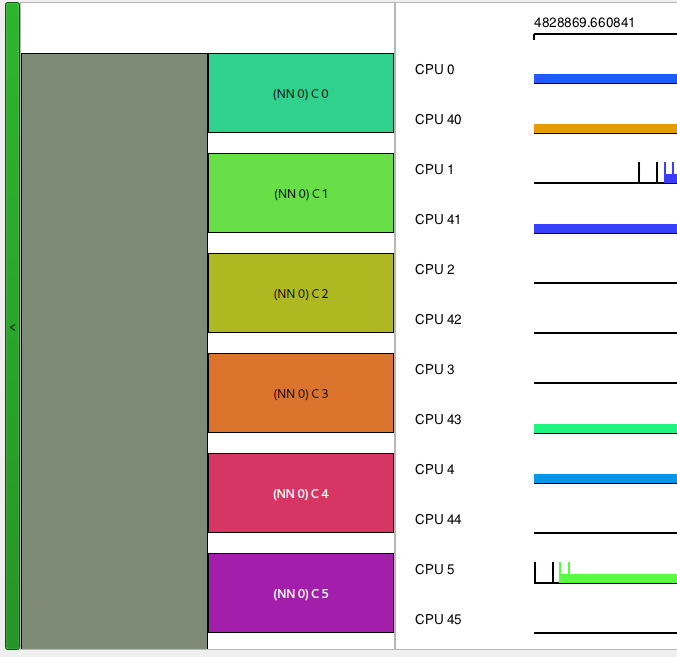
\includegraphics[width=140mm]{img/NUMATV/numatv-5}
    \caption{Viditelný topologický strom a zelené skrývající tlačítko vlevo}
    \label{numatv-5}
\end{figure}

\begin{figure}[p]\centering
    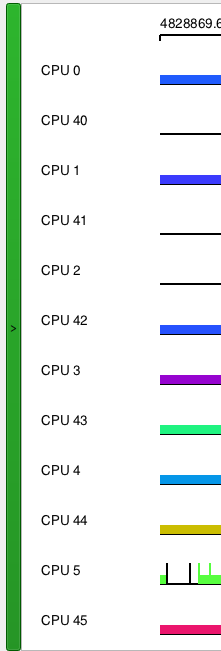
\includegraphics[height=180mm]{img/NUMATV/numatv-6}
    \caption{Skrytá plocha pro zobrazení topologií a zelené skrývající tlačítko vlevo}
    \label{numatv-6}
\end{figure}

\subsubsection{Topologický strom}

Topologický strom je blokový strom, který je zobrazen od prvního CPU grafu až po poslední CPU graf nějakého streamu v GL ploše grafů trasování. Pokud je otevřeno více streamů, které navíc vyžadují stromový pohled ve své konfiguraci, pak každý strom začíná u prvního CPU grafu svého streamu.

Součástí vykresleného topologického stromu jsou pouze vrcholy pro NUMA uzly a jádra, kterých jsou CPU z grafu součástí. Pokud tedy některé CPU grafy schováme, tak i zmenšíme zobrazení stromu na relevantní části topologie, tj. ty, které obsahují CPU viditelných CPU grafů. Topologický strom lze rozdělit na dvě vrstvy, na \uv{C} vrstvu pro jádra a \uv{NN} vrstvu pro NUMA uzly. Strom je navíc zobrazen tak, že vrstvy jdou zleva doprava a vpravo od topologické plochy jsou CPU grafy. Pak můžeme plynulým pohledem zprava doleva zjistit, jakému jádru CPU patří a i jakému NUMA uzlu. Vrstva NN je schována, pokud by byl zobrazen pouze jeden vrchol z této vrstvy, tj. všechna CPU v grafu trasování náleží jednomu NUMA uzlu.

Vrcholy/bloky topologického stromu jsou vždy zabarveny průměrnou barvou svých přímých pravých následníků. Vrcholy pro jádra získávají barvu CPU z KernelSharku. Značka každého vrcholu je buď černý nebo bílý text. To je dáno světlostí použité barvy bloku.

Značky ve vrcholech topologického stromu jsou zkratky NN, nebo C, dané vrstvou stromu, které vrchol patří. Vedle nich je pak zobrazen i logický index prvku topologie v této vrstvě. Dohromady pak text unikátně značí prvek v topologii. Pokud je NN vrstva viditelná, přidává se před značku vrcholu jádrové vrstvy do závorek značka vrcholu NUMA uzlu, který vlastní jádro tohoto vrcholu. Pokud přejedeme myší přes vrchol v topologickém stromě, zobrazí se nám plovoucí vysvětlivka, ve které je delší název pro vrchol. Například pro vrchol označený \uv{(NN 1) C 34} se zobrazí \uv{Core 34 in NUMA Node 1}, nebo pro \uv{NN 3} se zobrazí \uv{NUMA Node 3}. Obrázek \ref{numatv-8} ukazuje vysvětlivky při práci.

\begin{figure}[p]\centering
    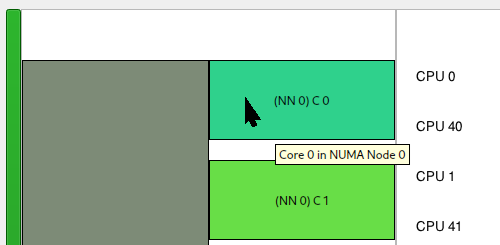
\includegraphics[width=140mm]{img/NUMATV/numatv-8}
    \caption{Vysvětlivka zobrazená při přejetí kurzoru myši nad vrcholem v topologickém stromu}
    \label{numatv-8}
\end{figure}

\subsubsection{Přeuspořádání CPU grafů}

Je možné, že topologický strom očekává pro svou strukturu jiné uspořádání CPU grafů, než jaké by KernelShark obyčejně provedl. Obyčejně, tj. i ve výchozím pohledu, KernelShark uspořádá CPU dle indexů, které získaly od operačního systému. U stromového pohledu jsou uspořádány pomocí logických indexů svých a prvků topologie, kterým patří. Nejprve se třídí podle logického indexu NUMA uzlu, pak podle logického indexu jádra a až poté podle logického indexu CPU. Setříděná sekvence by pak mohla vypadat následovně jako (0, 0, 0), (0, 0, 4), (0, 1, 1), (1, 2, 2), (1, 2, 3), kde složky třetice jsou právě logické indexy (první jsou NUMA uzly, pak jádra, pak procesory/CPU).

V CPU grafech a zbytku KernelSharku se stále používají OS indexy pro CPU. Pokud jsou logické indexy stejné jako OS indexy, pak uspořádání CPU grafů nemění.

Reorganizací CPU grafů jednoho streamu nevynutíme reorganizaci CPU grafů jiného streamu.

Znázorníme situaci reorganizace na obrázcích. Obrázek \ref{numatv-4} zobrazuje výchozí řazení podle OS indexů. Obrázek \ref{numatv-5} má grafy kvůli topologickému stromu přeuspořádané.

\begin{figure}[p]\centering
    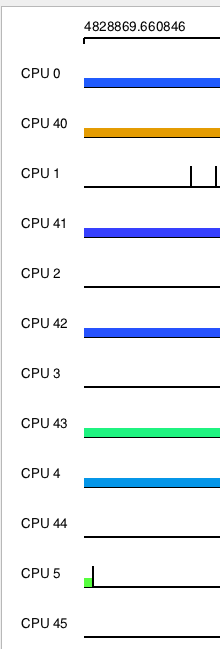
\includegraphics[height=180mm]{img/NUMATV/numatv-4}
    \caption{Výchozí řazení CPU grafů podle OS indexů}
    \label{numatv-4}
\end{figure}

\subsection{Podpora relací}

Konfigurace streamů pro NUMA~TV mohou být uloženy do relací. Každý stream má pak v relačních datech uložen vybraný pohled a cestu k topologickému souboru. Importováním relace se automaticky nakreslí i topologické stromy, žádají-li to nějaké streamy.

\subsection{Bugy a chyby}

Jediný bug, o kterém autor ví, je že při načítání relace s aktivní NUMA TV je možné, že se nezobrazí celý topologický strom pro stream, tj. některá poslední CPU nebudou pokryta tímto stromem. Příčina ani řešení nejsou známy.

%%%%%%%%%%%%%%%%%%%%%%%%%%%%%%%%%%%%%%%%%%%%%%%%%%%%%%%%%%%%%%%%%%%%%%%
\section{Rozšíření}
Tato sekce představí některá rozšíření, která by modifikaci zjednodušila, nebo by dodala nové funkce. Upozorňujeme, že se mohou objevit rozšíření, která upravují čistě implementaci, například zlepšují čitelnost kódu - u těchto se očekává znalost kódu vylepšení. Takové části budou vždy označeny v první větě jejich sekce.

\subsubsection*{Více pohledů}
NUMA~TV dokáže v současnosti zobrazit pouze topologii, která dělí systém, tj. stroj, podle NUMA uzlů, jader a procesorů. Ačkoliv je modifikace hůře rozšiřitelná (viz kritika o rozšiřitelnosti \ref{rozšiřitelnost}), šlo by s trochou práce přidat další pohledy a další vizualizace topologie. Jednou z možností je zobrazení topologie procesorových modulů, kde by se namísto NUMA uzlů použily procesorové moduly. Tím bychom mohli například zjistit, který z nich je nejvíc namáhaný. Navíc by šlo k této vizualizaci opět použít nějaký strom, klidně i nějaký odlišný od blokového.

\subsubsection*{Skládání částí stromu}
Původně měly být stromy skladatelné, tj. kliknutím na vrchol ve stromu by byl vrchol skryt a grafy s ním spojené schovány, ale jelikož se nejednalo o zásadní funkcionalitu, nebyly dodány. To ale neznamená, že jej nelze doplnit. Nástinem řešení by bylo přidat akci na událost kliknutí levého tlačítka myši, kterou se aktivuje kód podobný tomu, který je spuštěn při schování CPU grafů přes dialog, kterým bychom skryli jak CPU grafy, tak i bloky stromu topologie. Pak by bylo ještě nutné dodat nějaký grafický prvek pro schované vrcholy do topologické plochy, kterým bychom schovaný blok opět zviditelnili.

Toto rozšíření se pojí s předchozím, jelikož by bylo i možné dodat něco jako \uv{stromový pohled +}, který by dělal to samé, co nynější stromový pohled, ale dodal by topologickému stromu schopnost být skládán.

\subsubsection*{Barva uzlů topologického stromu}
Barvení NUMA uzlů v topologickém stromu není v praxi moc hezké, jelikož barvy jader se smíchají většinou do hnědé nebo šedé. Možná by šlo najít lepší barvení, například dát blokům NUMA uzlů nějaké dobře oddělené barvy (pro tři uzly třeba červenou, zelenou a modrou) a barvy jader by se pak jen lišily odstínem této hlavní barvy, třeba by byly jejich bloky temnější s rostoucím logickým indexem.

\subsubsection*{Konfigurační dialogy by mohly být zobecněny}
(Tato úprava očekává znalost kódu implementace.)

Couplebreak i NUMA~TV mají velmi podobné konfigurační dialogy, viz obrázek \ref{perstream-cfg}. Kód pro každý vytváří separátní třídu, ale šlo by je sjednotit do jedné třídy, které bychom při konstrukci pro specifickou modifikaci předali chování tlačítka \texttt{Apply} a obsah konfigurací pro každý stream. Rozšíření by pak hlavně snížilo duplicitní kód, který tyto konfigurační dialogy sdílí, zároveň by ale i představovalo použitelný dialog pro případné další modifikace, které by se týkaly jednotlivých streamů.

\begin{figure}[p]\centering
    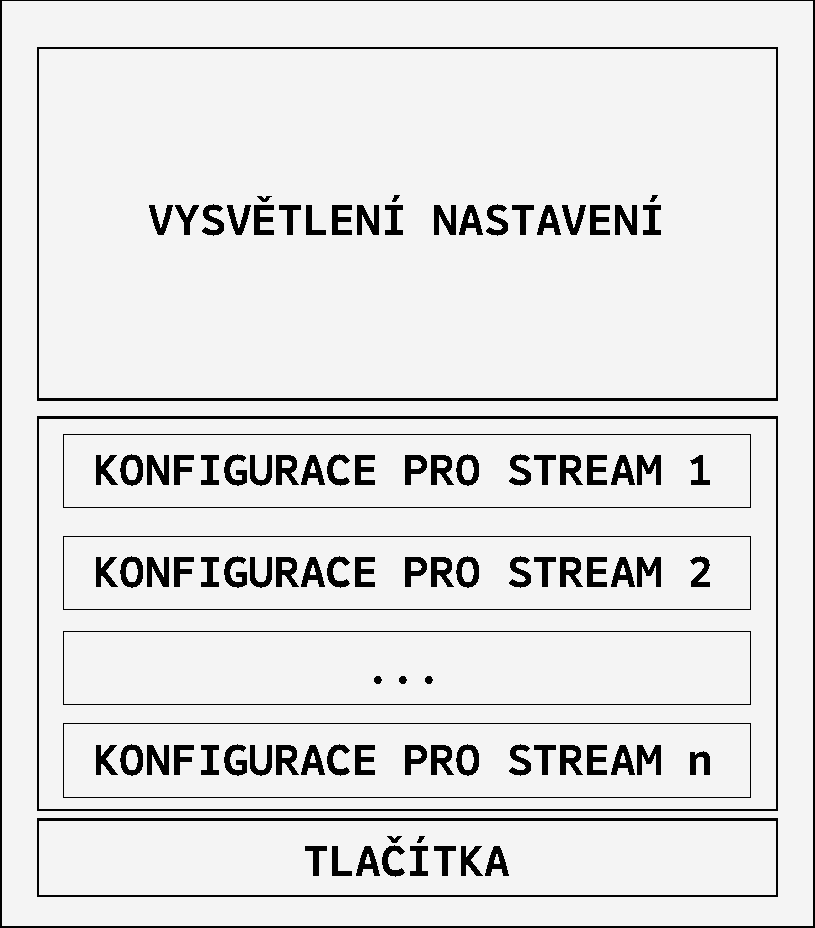
\includegraphics[width=140mm]{img/NUMATV/PerStreamCfg.pdf}
    \caption{Obecný formát konfiguračních dialogů pro NUMA~TV a Couplebreak.}
    \label{perstream-cfg}
\end{figure}

%%%%%%%%%%%%%%%%%%%%%%%%%%%%%%%%%%%%%%%%%%%%%%%%%%%%%%%%%%%%%%%%%%%%%%%
\section{Kritika}
V této sekci autor kriticky zhodnotí své řešení. Každá kritika má nadpis a popis a dále buď obsahuje obranu proti ní, nebo souhlas s předneseným problémem. Upozorňujeme, že se může objevit kritika, která se týká čistě implementace, tj. jenom toho, jak je řešení napsáno, nikoli řešení samotné. Taková kritika bude obsahovat v první větě svého popisu označení, že očekává znalost kódu implementace.

\subsubsection*{Nemožnost upravovat aktivní topologie}
V našem řešení se skoro nikdy neupravují konfigurace a vizualizace topologie, namísto toho se skoro vždy vytvoří nový objekt a starý se zahodí. To je hlavně dáno tím, že tyto operace se nedějí často, nemají tedy velkou ani časovou, ani prostorovou cenu, navíc je řešení pak jednodušší. Proto jsou pak akce úpravy často spíše akce smazání a přidání nových objektů.

\subsubsection*{Dialogy namísto standardních výstupů}
KernelShark sice používá standardní výstup na některé zprávy, nicméně bylo by možná lepší použít vyskakovací okénka pro NUMA~TV zprávy, které se nyní tisknou na standardní výstup či standardní chybový výstup. Se standardními výstupy se lépe pracuje, proto byly zvoleny, nicméně pro dokonalejší řešení by byly grafické zprávy lepší, alespoň pro zprávy informačního typu.

\subsubsection*{Topologie jako součást datové struktury streamu}
Je možné se zamyslet nad tím, proč není NUMA~TV konfigurace součástí datové struktury streamů jako Couplebreak, je-li na ně silně vázána. To je férová kritika a tento přístup by mohl fungovat. Přístup se samostatnými konfiguracemi byl zvolen jelikož streamy byly navrženy jako zdroje dat a metadat trasovaní. Couplebreak pak k těmto datům mohl přidat  kontrolní proměnné, které vylepšily dělení trasovacích dat. Vedle toho NUMA~TV modifikace není s trasováním prakticky tak spojená, jenom chce ukázat topologii systému vedle trasování, aby mohl uživatel příjemněji analyzovat chování systému v jednom programu. Identifikátory streamů používá hlavně pro navázání topologických stromů na CPU grafy, ale trasování a jeho data ji už tak moc nezajímají.

\subsubsection*{Rozšiřitelnost}
\label{rozšiřitelnost}
(Tato kritika očekává znalost kódu implementace.)

Současná implementace NUMA~TV není tak snadno rozšiřitelná, jak by mohla být. Pokud chceme zobrazit další topologie, tak nestačí pouze přidání nových pohledů, typů vizualizace a propojení s konfigurací, jelikož modifikace očekává třídy specifické pro NUMA topologie.

Více rozšiřitelné řešení by mohlo mít nějaké rodičovské třídy pro vizualizace a konfigurace, se kterými by pracoval zbytek KernelSharku, vedle nových pohledů a tlačítek v konfiguraci. Třídy pro NUMA topologie by byly dětmi těchto rodičů a musely by splnit nějaká rozhraní, aby se jim správně zobrazovaly jejich stromy.

%%%%%%%%%%%%%%%%%%%%%%%%%%%%%%%%%%%%%%%%%%%%%%%%%%%%%%%%%%%%%%%%%%%%%%%
\section{Zhodnocení splnění požadavků}
Modifikace není u žádného z otevřených streamů aktivní, dokud není zapnuta skrze konfigurační dialog. Uživatel tak vůbec o NUMA~TV při práci vědět nemusí, může si maximálně všimnout tlačítka, kterým právě zapne konfigurační dialog. Navíc, pokud soubor s relačními daty neobsahuje data pro NUMA~TV, tak bude modifikace jednoduše používat výchozí hodnoty, program kvůli tomu nespadne ani nenahlásí chybu. Tím splňujeme obecný požadavek \emph{minimálního vlivu}. NUMA~TV se dá označit za úplně nový modul pro KernelShark, navíc jenom rozšiřuje chování u míst, kde byly modifikovány původní funkce a struktury, nemění jejich původní záměry. Takže splňuje i obecný požadavek \emph{chování se jako rozšíření}. Obecný požadavek na \emph{stylovou podobnost} se musí ověřit čtením kódu provedených změn, nicméně rychle lze například nahlédnout, že NUMA~TV používá stejné velikosti písmen pro třídy jako zbytek KernelSharku.

Vlastní požadavky, tj. cíle, jsme splnili navržením řešení v analýze právě podle nich.